\section{Method}


\subsection{Singularity}
To complete the workflow from raw data to protein quantification results, several other software had to be included in the container.

There are a multitude of different types of MS data types, each of which has different file formats which are incompatible with Quandenser. To combat the problem, a software named \textit{Msconvert} was added to the workflow, which can convert MS data from a multitude of vendor formats to a general MS data format. Due to conversion from vendor formats with Msconvert only works with the distribution released for the Windows operative system, while the Singularity image was based on Ubuntu, a Linux operative system, another method was required to make Msconvert work within the image. The solution was utilizing another type of emulator software, named \textit{Wine}, which can emulate a Windows environment inside a Linux environment.

Bayesian method, Triqler

\subsection{Nextflow}

\begin{comment}
% Right aling
\begin{wrapfigure}{r}{5.5cm}
  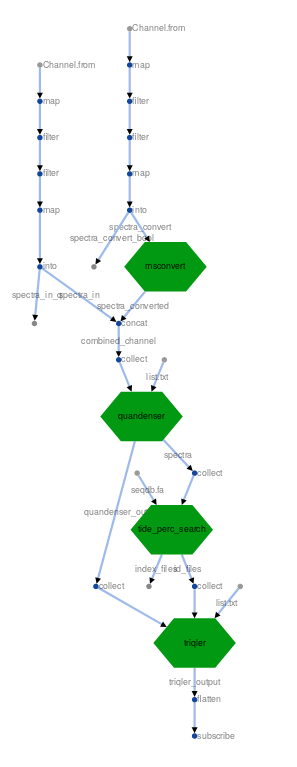
\includegraphics[width=7cm, height=15cm]{pictures/workflow.png}
  \caption{Workflow of the pipeline}
  \label{fig:workflow}
\end{wrapfigure}
\end{comment}


\subsection{Quandenser-pipeline GUI}


\subsection{Analysing bacterial proteomes}

Comparison between established methods, which uses similar workflow management systems were also compared to the created workflow pipeline. Another workflow manager \textit{KNIME} in combination with \textit{OpenMS} was used to compare
After Quandenser has
